% ==========================================
% BAB IV PERANCANGAN
% ==========================================
\cleardoublepage
\chapter{PERANCANGAN ARSITEKTUR DAN INTERAKSI SISTEM}
\label{chap:perancangan}

Bab ini menguraikan rancangan konsep solusi yang diusulkan melalui dua perspektif pemodelan utama: pemodelan konteks dan interaksi untuk menggambarkan batasan dan fungsionalitas sistem, serta pemodelan struktur dan perilaku untuk merinci mekanisme kolaborasi antarkomponen internal.

\section{Model Konteks dan Interaksi (\textit{Use Case Diagram})}
\label{sec:context_interaction_model}
Model ini mendefinisikan batasan sistem (\textit{system boundary}),
mana saja yang menjadi fitur yang diimplementasikan di dalam sistem
dan mana saja yang berada di luar sistem, terutama aktor.
Selain itu, bisa dijelaskan juga interaksi yang terjadi antara aktor
eksternal dengan fitur-fitur utama sistem.

\textit{Use case} didefinisikan berdasarkan pemetaan terhadap
kebutuhan fungsional yang telah diuraikan pada Subbab \ref{sec:analisis_kebutuhan}, sebagaimana dapat dilihat pada Tabel \ref{tbl:mapping_fr_uc}.

\input{tables/tabel_4_mapping_fr_uc.tex}

Penggambaran dari setiap \textit{use case} di atas dan interaksinya dengan aktor
luar, tercermin pada gambar \ref{fig:usecase_model} di bawah ini.

\begin{figure}[!ht]
    \centering
    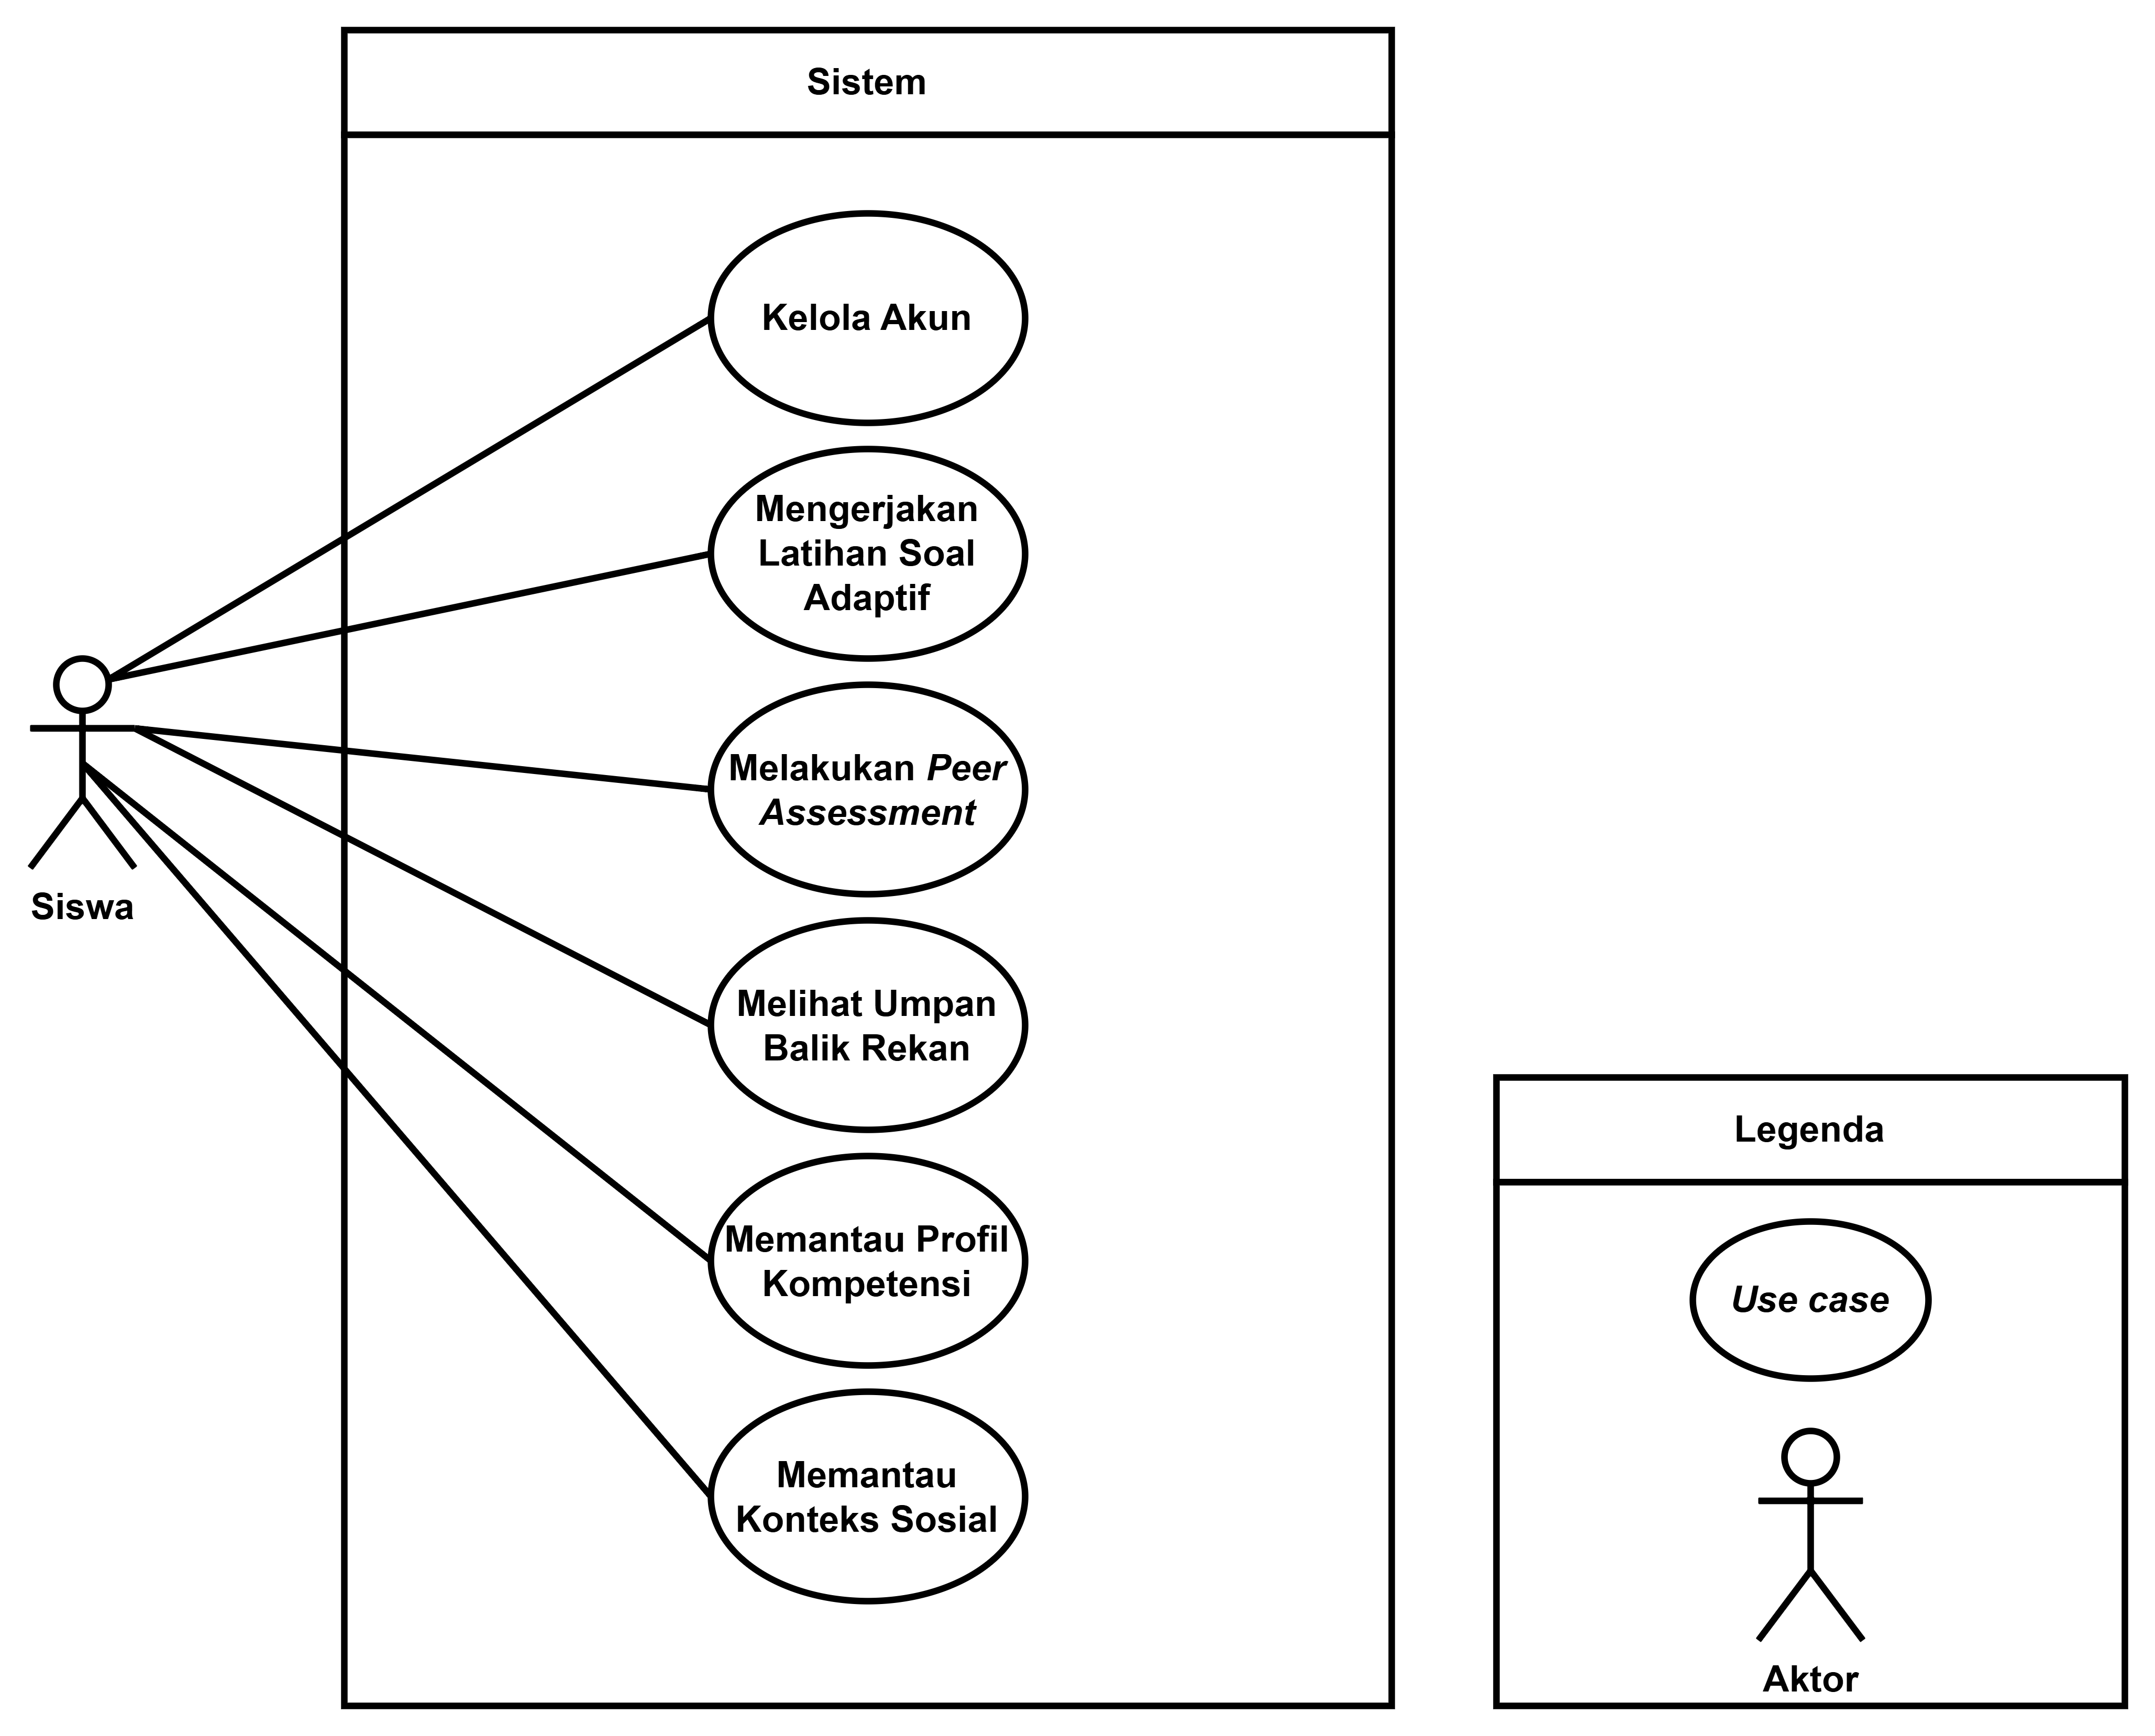
\includegraphics[width=0.8\textwidth]{images/usecase_diagram.png}
    \caption{\textit{Use Case Diagram} - Interaksi pemelajar dengan Sistem}
    \label{fig:usecase_model}
\end{figure}

Adapun penjelasan dari setiap \textit{use case} secara lebih terperinci disajikan
pada tabel-tabel berikut ini.

% --- Tabel Deskripsi UC-01 ---
\begin{table}[H]
    \centering
    \caption{Deskripsi \textit{Use Case} Kelola Akun (UC-01)}
    \label{tbl:desc_uc01}
    \begin{tabular}{|p{0.20\textwidth}|p{0.70\textwidth}|}
        \hline
        \textbf{Nama \textit{Use Case}} & \textbf{Kelola Akun} \\
        \hline
        \textbf{Aktor} & pemelajar \\
        \hline
        \textbf{FR Terkait} & FR-01 \\
        \hline
        \textbf{Deskripsi} & Proses autentikasi pengguna untuk memastikan keamanan akses terhadap data profil kompetensi dan riwayat pembelajaran. \\
        \hline
        \textbf{Kondisi sebelum} & pemelajar memiliki akun yang terdaftar di dalam basis data sistem. \\
        \hline
        \textbf{Kondisi sesudah} & Sesi pengguna aktif; Sistem memuat profil Elo rating pemelajar. \\
        \hline
        \textbf{Main Flow} & \begin{enumerate}[noitemsep,topsep=0pt,leftmargin=*]
            \item pemelajar memasukkan kredensial akun (\textit{username/password}).
            \item Sistem memvalidasi kesesuaian data.
            \item Sistem menginisialisasi sesi pembelajaran.
            \item Sistem menampilkan dasbor utama.
        \end{enumerate} \\
        \hline
    \end{tabular}
\end{table}
% --- Tabel Deskripsi UC-02 ---
\begin{table}[H]
    \centering
    \caption{Deskripsi \textit{Use Case} Mengerjakan Latihan Adaptif (UC-02)}
    \label{tbl:desc_uc02}
    \begin{tabular}{|p{0.20\textwidth}|p{0.70\textwidth}|}
        \hline
        \textbf{Nama \textit{Use Case}} & \textbf{Mengerjakan Latihan Adaptif} \\
        \hline
        \textbf{Aktor} & pelajar \\
        \hline
        \textbf{FR Terkait} & FR-02, FR-08 \\
        \hline
        \textbf{Deskripsi} & pelajar mengerjakan soal latihan yang dipilihkan secara dinamis oleh sistem berdasarkan estimasi kemampuan saat ini untuk meningkatkan kompetensi. \\
        \hline
        \textbf{Kondisi sebelum} & pelajar telah login; Nilai parameter Elo rating ($\theta$) pelajar tersedia. \\
        \hline
        \textbf{Kondisi sesudah} & Skor Elo pelajar diperbarui; Sistem mengevaluasi tren variabilitas skor (deteksi stagnasi). \\
        \hline
        \textbf{Main Flow} & \begin{enumerate}[noitemsep,topsep=0pt,leftmargin=*]
            \item Sistem memilih latihan soal dengan tingkat kesulitan setara ($D_j \approx R_i$).
            \item Sistem menampilkan soal kepada pelajar.
            \item pelajar menginputkan jawaban.
            \item Sistem memvalidasi jawaban dan menghitung skor aktual.
            \item Sistem memperbarui profil kompetensi pelajar.
        \end{enumerate} \\
        \hline
    \end{tabular}
\end{table}
% --- Tabel Deskripsi UC-03 ---
\begin{table}[H]
    \centering
    \caption{Deskripsi \textit{Use Case} Melakukan \textit{Peer Assessment} (UC-03)}
    \label{tbl:desc_uc03}
    \begin{tabular}{|p{0.20\textwidth}|p{0.70\textwidth}|}
        \hline
        \textbf{Nama \textit{Use Case}} & \textbf{Melakukan \textit{Peer Assessment}} \\
        \hline
        \textbf{Aktor} & pelajar \\
        \hline
        \textbf{FR Terkait} & FR-03, FR-09 \\
        \hline
        \textbf{Deskripsi} & pelajar mengevaluasi pekerjaan rekan sejawat menggunakan rubrik terstruktur. Aktivitas ini dipicu oleh sistem untuk memecahkan isolasi kompetensi. \\
        \hline
        \textbf{Kondisi sebelum} & Sistem mendeteksi stagnasi pembelajaran; Algoritma \textit{Re-ranking} telah menemukan pasangan heterogen. \\
        \hline
        \textbf{Kondisi sesudah} & Skor Elo \textit{Assessee} diperbarui (berdasarkan nilai tugas); Skor Elo \textit{Assessor} diperbarui (berdasarkan kualitas reviu). \\
        \hline
        \textbf{Main Flow} & \begin{enumerate}[noitemsep,topsep=0pt,leftmargin=*]
            \item pelajar menerima notifikasi tugas \textit{peer-assessment}.
            \item Sistem menampilkan jawaban rekan \textbf{tanpa identitas (anonim)} beserta kolom penilaian.
            \item pelajar mengisi penilaian.
            \item Sistem memproses hasil untuk memperbarui Elo rating kedua belah pihak.
        \end{enumerate} \\
        \hline
    \end{tabular}
\end{table}
\input{tables/tabel_4_uc04.tex}
% --- Tabel Deskripsi UC-05 ---
\begin{table}[H]
    \centering
    \caption{Deskripsi \textit{Use Case} Memantau Profil Kompetensi (UC-05)}
    \label{tbl:desc_uc05}
    \begin{tabular}{|p{0.20\textwidth}|p{0.70\textwidth}|}
        \hline
        \textbf{Nama \textit{Use Case}} & \textbf{Memantau Profil Kompetensi} \\
        \hline
        \textbf{Aktor} & Siswa \\
        \hline
        \textbf{FR Terkait} & FR-05, FR-06, FR-07 \\
        \hline
        \textbf{Deskripsi} & Siswa melihat visualisasi perkembangan kemahiran individunya, termasuk kontribusi dari aktivitas individu dan sosial. \\
        \hline
        \textbf{Kondisi sebelum} & Data riwayat aktivitas pembelajaran siswa tersedia. \\
        \hline
        \textbf{Kondisi sesudah} & Informasi profil ditampilkan. Tidak ada perubahan data. \\
        \hline
        \textbf{Main Flow} & \begin{enumerate}[noitemsep,topsep=0pt,leftmargin=*]
            \item Siswa mengakses menu profil.
            \item Sistem mengambil data skor Elo milik siswa.
            \item Sistem menampilkan data skor Elo terkini.
            \item Sistem menampilkan juga data skor sosial.
        \end{enumerate} \\
        \hline
    \end{tabular}
\end{table}
% --- Tabel Deskripsi UC-06 ---
\begin{table}[H]
    \centering
    \caption{Deskripsi Use Case Memantau Konteks Sosial (UC-06)}
    \label{tbl:desc_uc06}
    \begin{tabular}{|p{0.20\textwidth}|p{0.70\textwidth}|}
        \hline
        \textbf{Nama Use Case} & \textbf{Memantau Konteks Sosial} \\
        \hline
        \textbf{Aktor} & pelajar \\
        \hline
        \textbf{FR Terkait} & FR-04 \\
        \hline
        \textbf{Deskripsi} & pelajar melihat posisi relatif kemahirannya dibandingkan dengan distribusi kemampuan kelas secara anonim (\textit{Social Awareness}). \\
        \hline
        \textbf{Kondisi sebelum} & Data agregat kemampuan seluruh kelas tersedia. \\
        \hline
        \textbf{Kondisi sesudah} & Visualisasi distribusi kelas ditampilkan. \\
        \hline
        \textbf{Main Flow} & \begin{enumerate}[noitemsep,topsep=0pt,leftmargin=*]
            \item pelajar mengakses menu wawasan grup/kelas.
            \item Sistem mengagregasi data pengguna aktif.
            \item Sistem menampilkan distribusi nilai grup/kelas.
        \end{enumerate} \\
        \hline
    \end{tabular}
\end{table}

Berdasarkan pemodelan \textit{use case} yang telah dijelaskan di atas, karakteristik interaksi sistem yang
diusulkan menunjukkan pergeseran dari paradigma sistem yang pasif menjadi sistem dengan intervensi aktif.
Perbedaan utamanya terletak pada mekanisme intervensi yang diinisiasi dari sistem, khususnya pada UC-03.
Berbeda dengan sistem yang sudah ada seperti UCRS dan OSSM yang mengandalkan motivasi atau kesadaran pemelajar untuk
melakukan kolaborasi, sistem yang diusulkan ini akan secara proaktif memantau kondisi model kompetensi pemelajar
melalui hasil algoritma \textit{Elo rating}. Ketika terjadi stagnasi dalam perubahan skor, maka sistem akan mendorong
aktivitas kolaboratif sebagai respons otomatis. Hal ini memperluas cakupan sistem dari sekadar penyaji konten
pembelajaran adaptif menjadi fasilitator pembelajaran otonom yang menjamin terjadinya eksposur terhadap keberagaman kompetensi.

\section{Model Struktur dan Perilaku (Communication Diagram)}
\label{sec:structure_behavior_model}

Untuk memodelkan bagaimana komponen internal berkolaborasi dalam menjalankan logika asesmen adaptif, digunakan \textit{Communication Diagram} dengan pendekatan \textbf{\textit{Boundary-Control-Entity} (BCE)}.

Pemilihan pola analisis BCE didasarkan pada kesesuaiannya dalam menjembatani spesifikasi \textit{Use Case} (fungsionalitas) menuju perancangan komponen logis, dengan karakteristik sebagai berikut:
\begin{enumerate}
    \item \textbf{Abstraksi Konseptual:} Berbeda dengan pola arsitektur implementasi seperti MVC (\textit{Model-View-Controller}) yang terikat pada kerangka kerja teknis, BCE berfokus pada peran semantik objek dalam menyelesaikan skenario bisnis tanpa bias teknologi.
    \item \textbf{Pemisahan Logika Intervensi:} Pola ini secara eksplisit memisahkan objek \textit{Control} (pengendali alur logika) dari \textit{Entity} (data persisten). Hal ini krusial untuk menggambarkan letak algoritma \textit{Re-ranking} dan \textit{Elo rating} yang bertindak sebagai otak sistem, terpisah dari data profil pemelajar.
\end{enumerate}

Gambar \ref{fig:communication_diagram} memvisualisasikan kolaborasi objek menggunakan pola ini.

\begin{figure}[!ht]
    \centering
    % Placeholder gambar Communication Diagram
    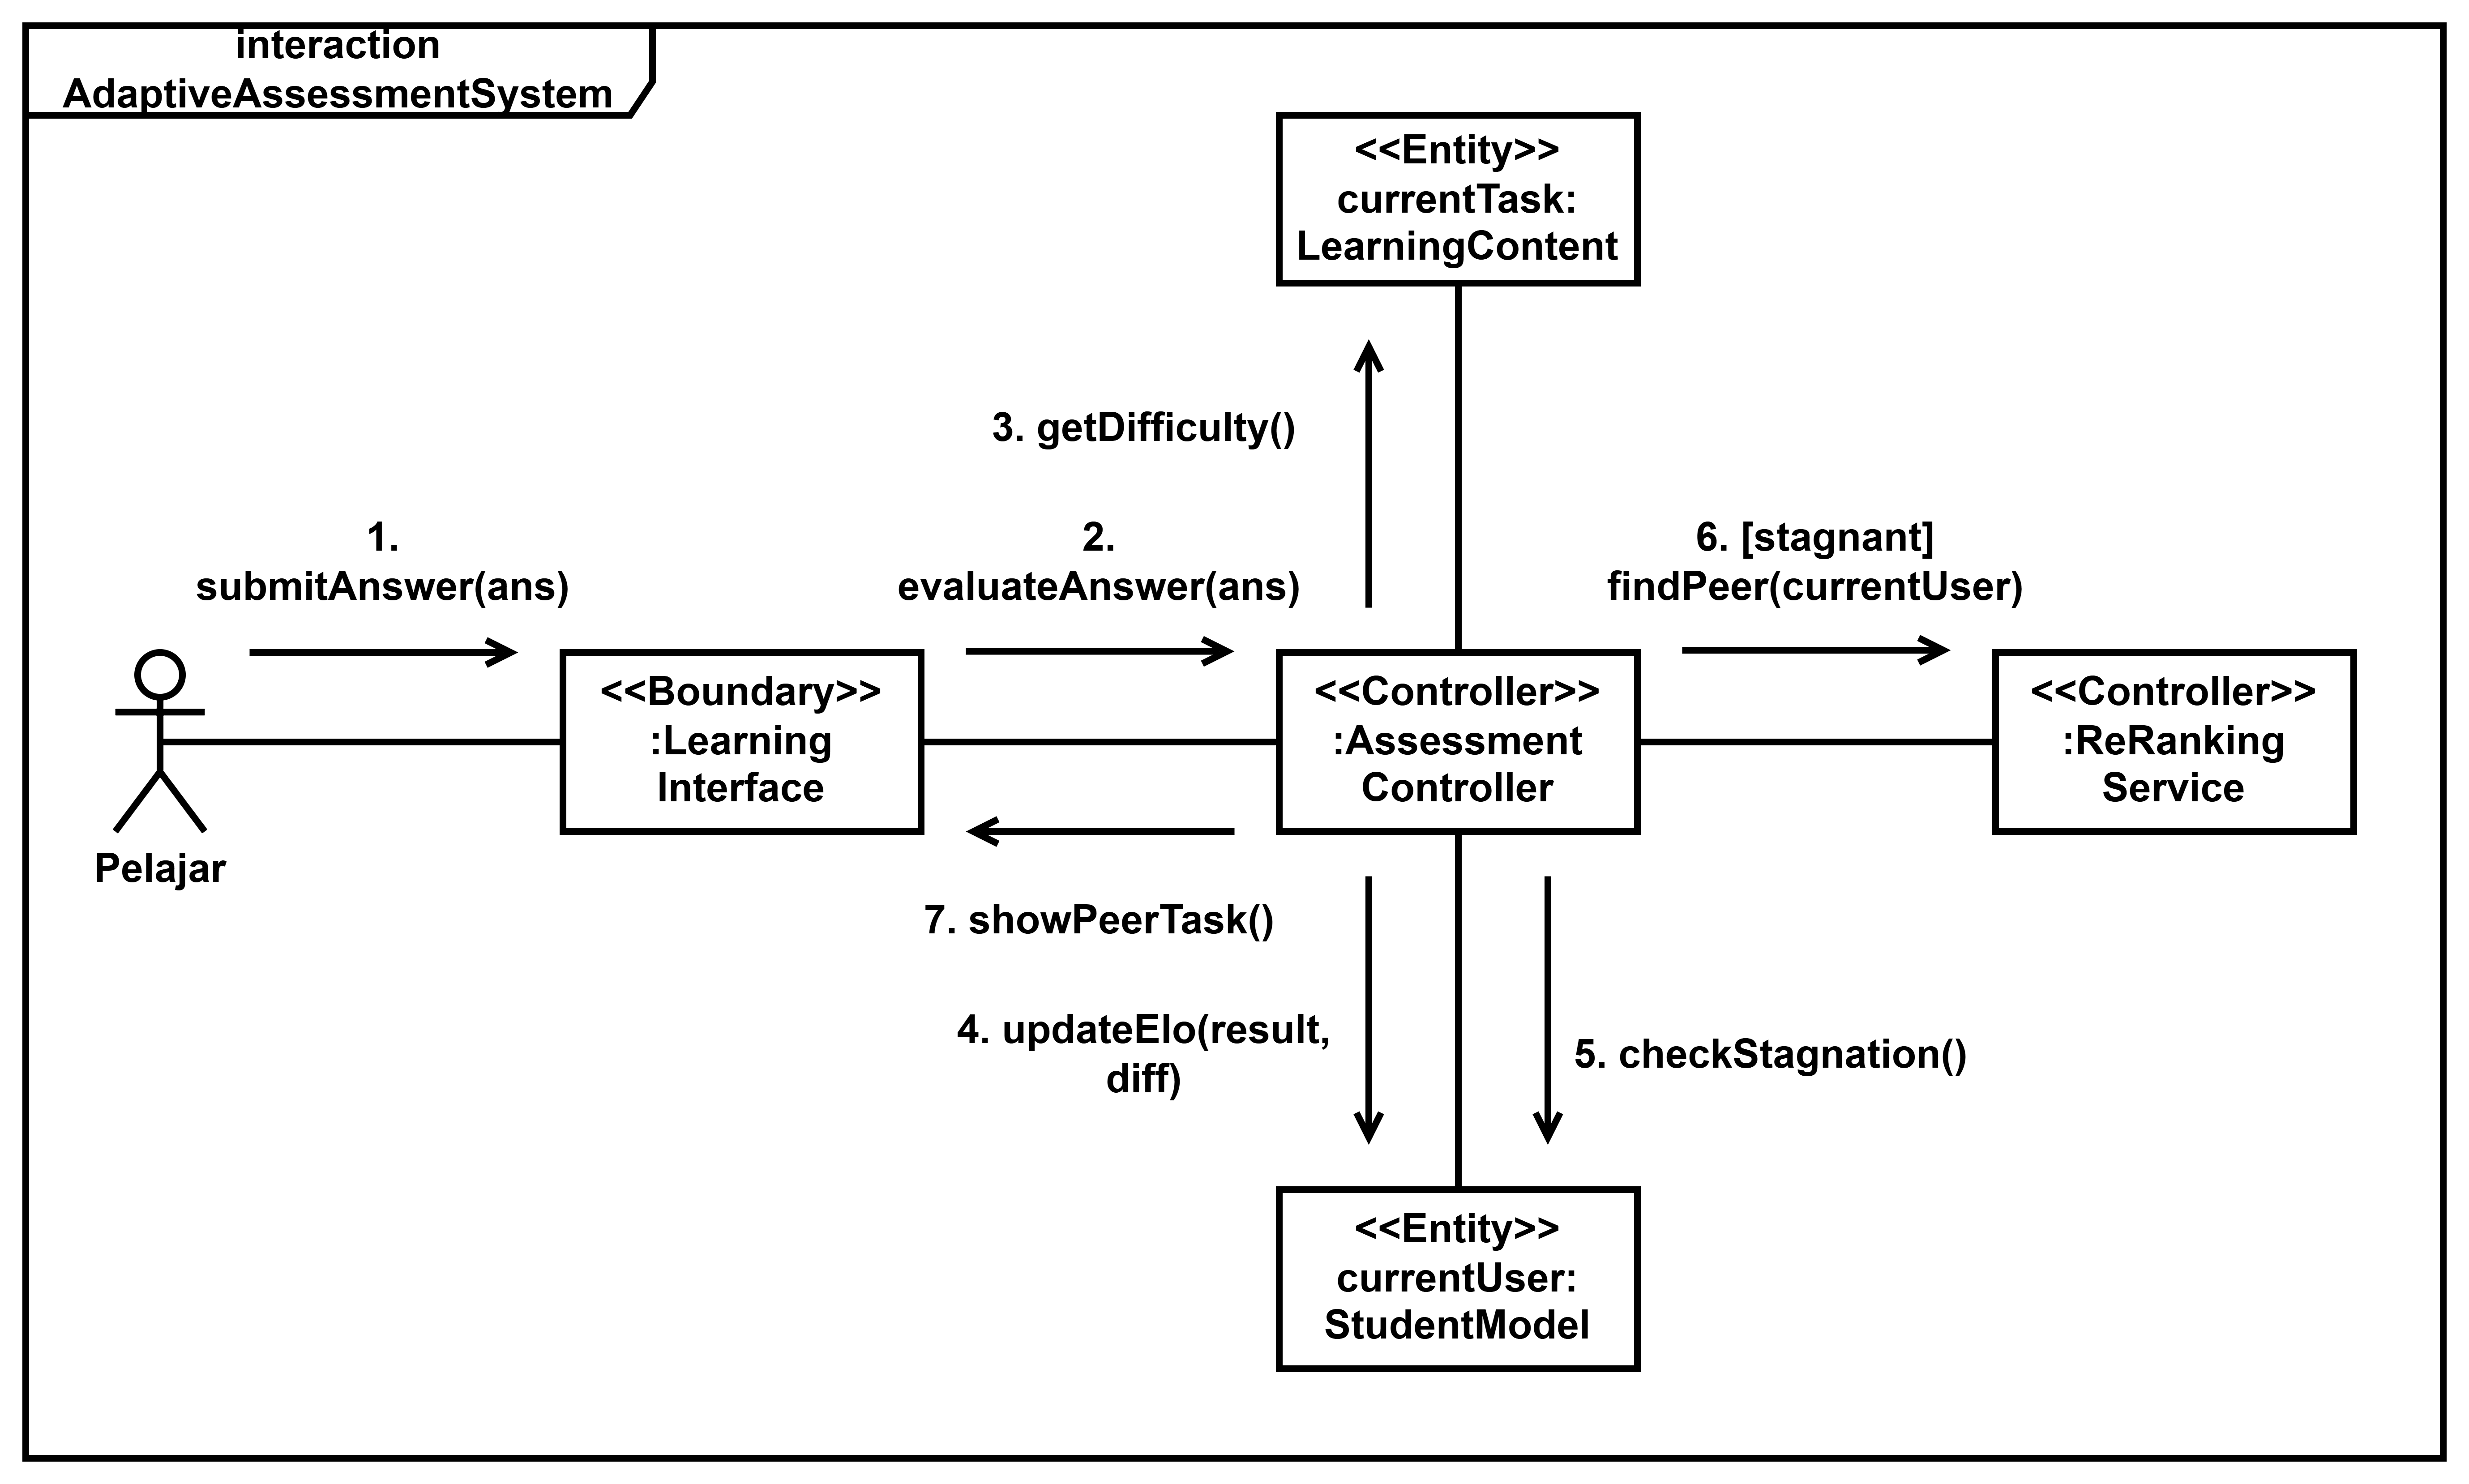
\includegraphics[width=1\textwidth]{images/communication_diagram.png}
    \caption{\textit{Communication Diagram} - Interaksi Komponen pada Sistem}
    \label{fig:communication_diagram}
\end{figure}

Diagram di atas menunjukkan interaksi yang diawali oleh Aktor \textbf{pemelajar} dan melibatkan kolaborasi tiga jenis objek analisis:

\begin{enumerate}
    \item \textbf{Boundary Object (\texttt{:LearningInterface}):} 
    Objek yang membatasi sistem dengan aktor luar. Bertanggung jawab menangkap pemicu kejadian (\textit{event}) berupa jawaban pemelajar dan menyajikan umpan balik visual.
    
    \item \textbf{Control Objects (\texttt{:AssessmentController} \& \texttt{:ReRankingService}):} 
    Objek pengendali yang merepresentasikan logika bisnis dinamis. 
    \begin{enumerate}
        \item \texttt{:AssessmentController} mengorkestrasi alur penilaian dan pengecekan kondisi stagnasi.
        \item \texttt{:ReRankingService} adalah objek kontrol yang secara spesifik mengenkapsulasi algoritma \textit{Constraint-based Re-ranking} \autocite{DeBiasio2023} untuk memproses logika seleksi mitra.
    \end{enumerate}
    
    \item \textbf{Entity Objects (\texttt{currentTask} \& \texttt{currentUser}):} 
    Objek yang merepresentasikan konsep data persisten yang berumur panjang. Objek ini menyimpan \textit{state} penting seperti parameter tingkat kesulitan soal ($D_j$) serta skor kemahiran pemelajar yang mencakup dimensi kemampuan individu dan kontribusi sosialnya dalam sistem. Data ini menjadi basis perhitungan utama bagi objek \textit{Control}.
\end{enumerate}

Alur pesan (\textit{Message Flow}) pada diagram menunjukkan bahwa interaksi tidak hanya terjadi antarmodul, melainkan melibatkan manipulasi langsung terhadap objek data (\textit{Entities}). Misalnya pesan \texttt{updateElo()} dikirimkan ke objek \texttt{currentUser}, dan pesan \texttt{getDifficulty()} diambil dari objek \texttt{currentTask}.

Alur pertukaran pesan pada Gambar \ref{fig:communication_diagram} dirancang untuk menangani transisi mulus antara aktivitas pengerjaan tugas individu dan intervensi sosial. Berikut adalah penjelasan rasionalisasi untuk setiap tahapan interaksi:

\begin{enumerate}
    \item \textbf{Inisiasi dan Evaluasi (Pesan 1-4):}
    Interaksi dimulai ketika aktor \textit{User} mengirimkan jawaban (\texttt{submitAnswer}) ke \texttt{:LearningInterface}. Antarmuka meneruskan data ke \texttt{:AssessmentController}, yang bertindak sebagai koordinator pusat. kontroler kemudian meminta atribut kesulitan ($D_j$) dari objek \texttt{currentTask} untuk menghitung probabilitas keberhasilan. Setelah perhitungan selesai, kontroler memerintahkan objek \texttt{currentUser} untuk memperbarui skor \textit{Elo}-nya (\texttt{updateElo}).
    
    \item \textbf{Deteksi Stagnasi (Pesan 5):}
    Segera setelah pembaruan skor, kontroler mengirim pesan \texttt{checkStagnation()} ke objek \texttt{currentUser}. 
    Langkah ini dirancang untuk mendeteksi fenomena \textit{learning plateau} \autocite{Halkiopoulos2024}, yaitu kondisi stagnasi pembelajaran akibat personalisasi berlebih. Deteksi dilakukan secara algoritmik dengan menghitung nilai variansi dari perubahan skor kemahiran $\theta$ (\textit{variance of} $\Delta\theta$) pada beberapa aktivitas terakhir. Jika nilai variansi berada di bawah ambang batas ($\epsilon$) tertentu, hal tersebut diinterpretasikan sebagai konvergensi prematur, yaitu kondisi yang mengindikasikan tantangan sistem sudah terlalu selaras dengan kemampuan pemelajar saat ini sehingga tidak lagi mendorong pertumbuhan kognitif.
    
    \item \textbf{Delegasi Mitigasi (Pesan 6):}
    Jika status stagnasi bernilai \textit{true}, kontroler tidak menangani pencarian rekan sendiri, melainkan mendelegasikannya ke objek \texttt{:ReRankingService} melalui pesan \texttt{findHeterogeneousPeer()}.
    Pemisahan ini dilakukan untuk mengisolasi logika algoritma \textit{Constraint-based Re-ranking} \autocite{DeBiasio2023} yang kompleks. Layanan ini bertanggung jawab menerapkan batasan statistik berdasarkan suatu pengukuran heterogenitas (seperti \textit{Cohen's d} $\geq 0.5$) untuk menyaring kandidat rekan. Hal ini memastikan bahwa rekan yang terpilih memiliki perbedaan tingkat kemampuan yang cukup signifikan untuk memecahkan stagnasi pembelajaran.
    
    \item \textbf{Eksekusi Intervensi (Pesan 7):}
    Setelah mendapatkan umpan balik yang valid, \texttt{:AssessmentController} akan mengirimkan pesan \texttt{showPeerTask()} ke \texttt{:LearningInterface}.
    Pesan ini secara dinamis mengubah mode tampilan antarmuka dari mode pengerjaan soal menjadi mode penilaian sejawat. Perubahan konteks yang diinisiasi sistem ini memaksa pemelajar untuk terlibat dalam aktivitas sosial tanpa perlu menavigasi menu secara manual, menjamin terjadinya eksposur terhadap perspektif baru.
\end{enumerate}

\section{Model Interaksi Detail (\textit{Sequence Diagram})}
\label{sec:sequence_diagram}

Berbeda dengan \textit{Communication Diagram} pada subbab sebelumnya yang berfokus pada peran logis objek secara konseptual, \textit{Sequence Diagram} memodelkan interaksi antarkomponen secara lebih detail dan spesifik dari segi arsitektur teknis. Diagram ini memetakan alur pertukaran pesan mulai dari antarmuka pengguna (\textit{Frontend}), layanan penyedia data (\textit{API Service}), berbagai mesin komputasi algoritma (\textit{Engines}), hingga ke basis data (\textit{Database}).

Gambar \ref{fig:sequence_diagram} mengilustrasikan keseluruhan siklus interaksi asesmen pemelajar, mulai dari pengerjaan soal hingga terjadinya intervensi kolaboratif apabila stagnasi terdeteksi. 

\begin{figure}[!ht]
    \centering
    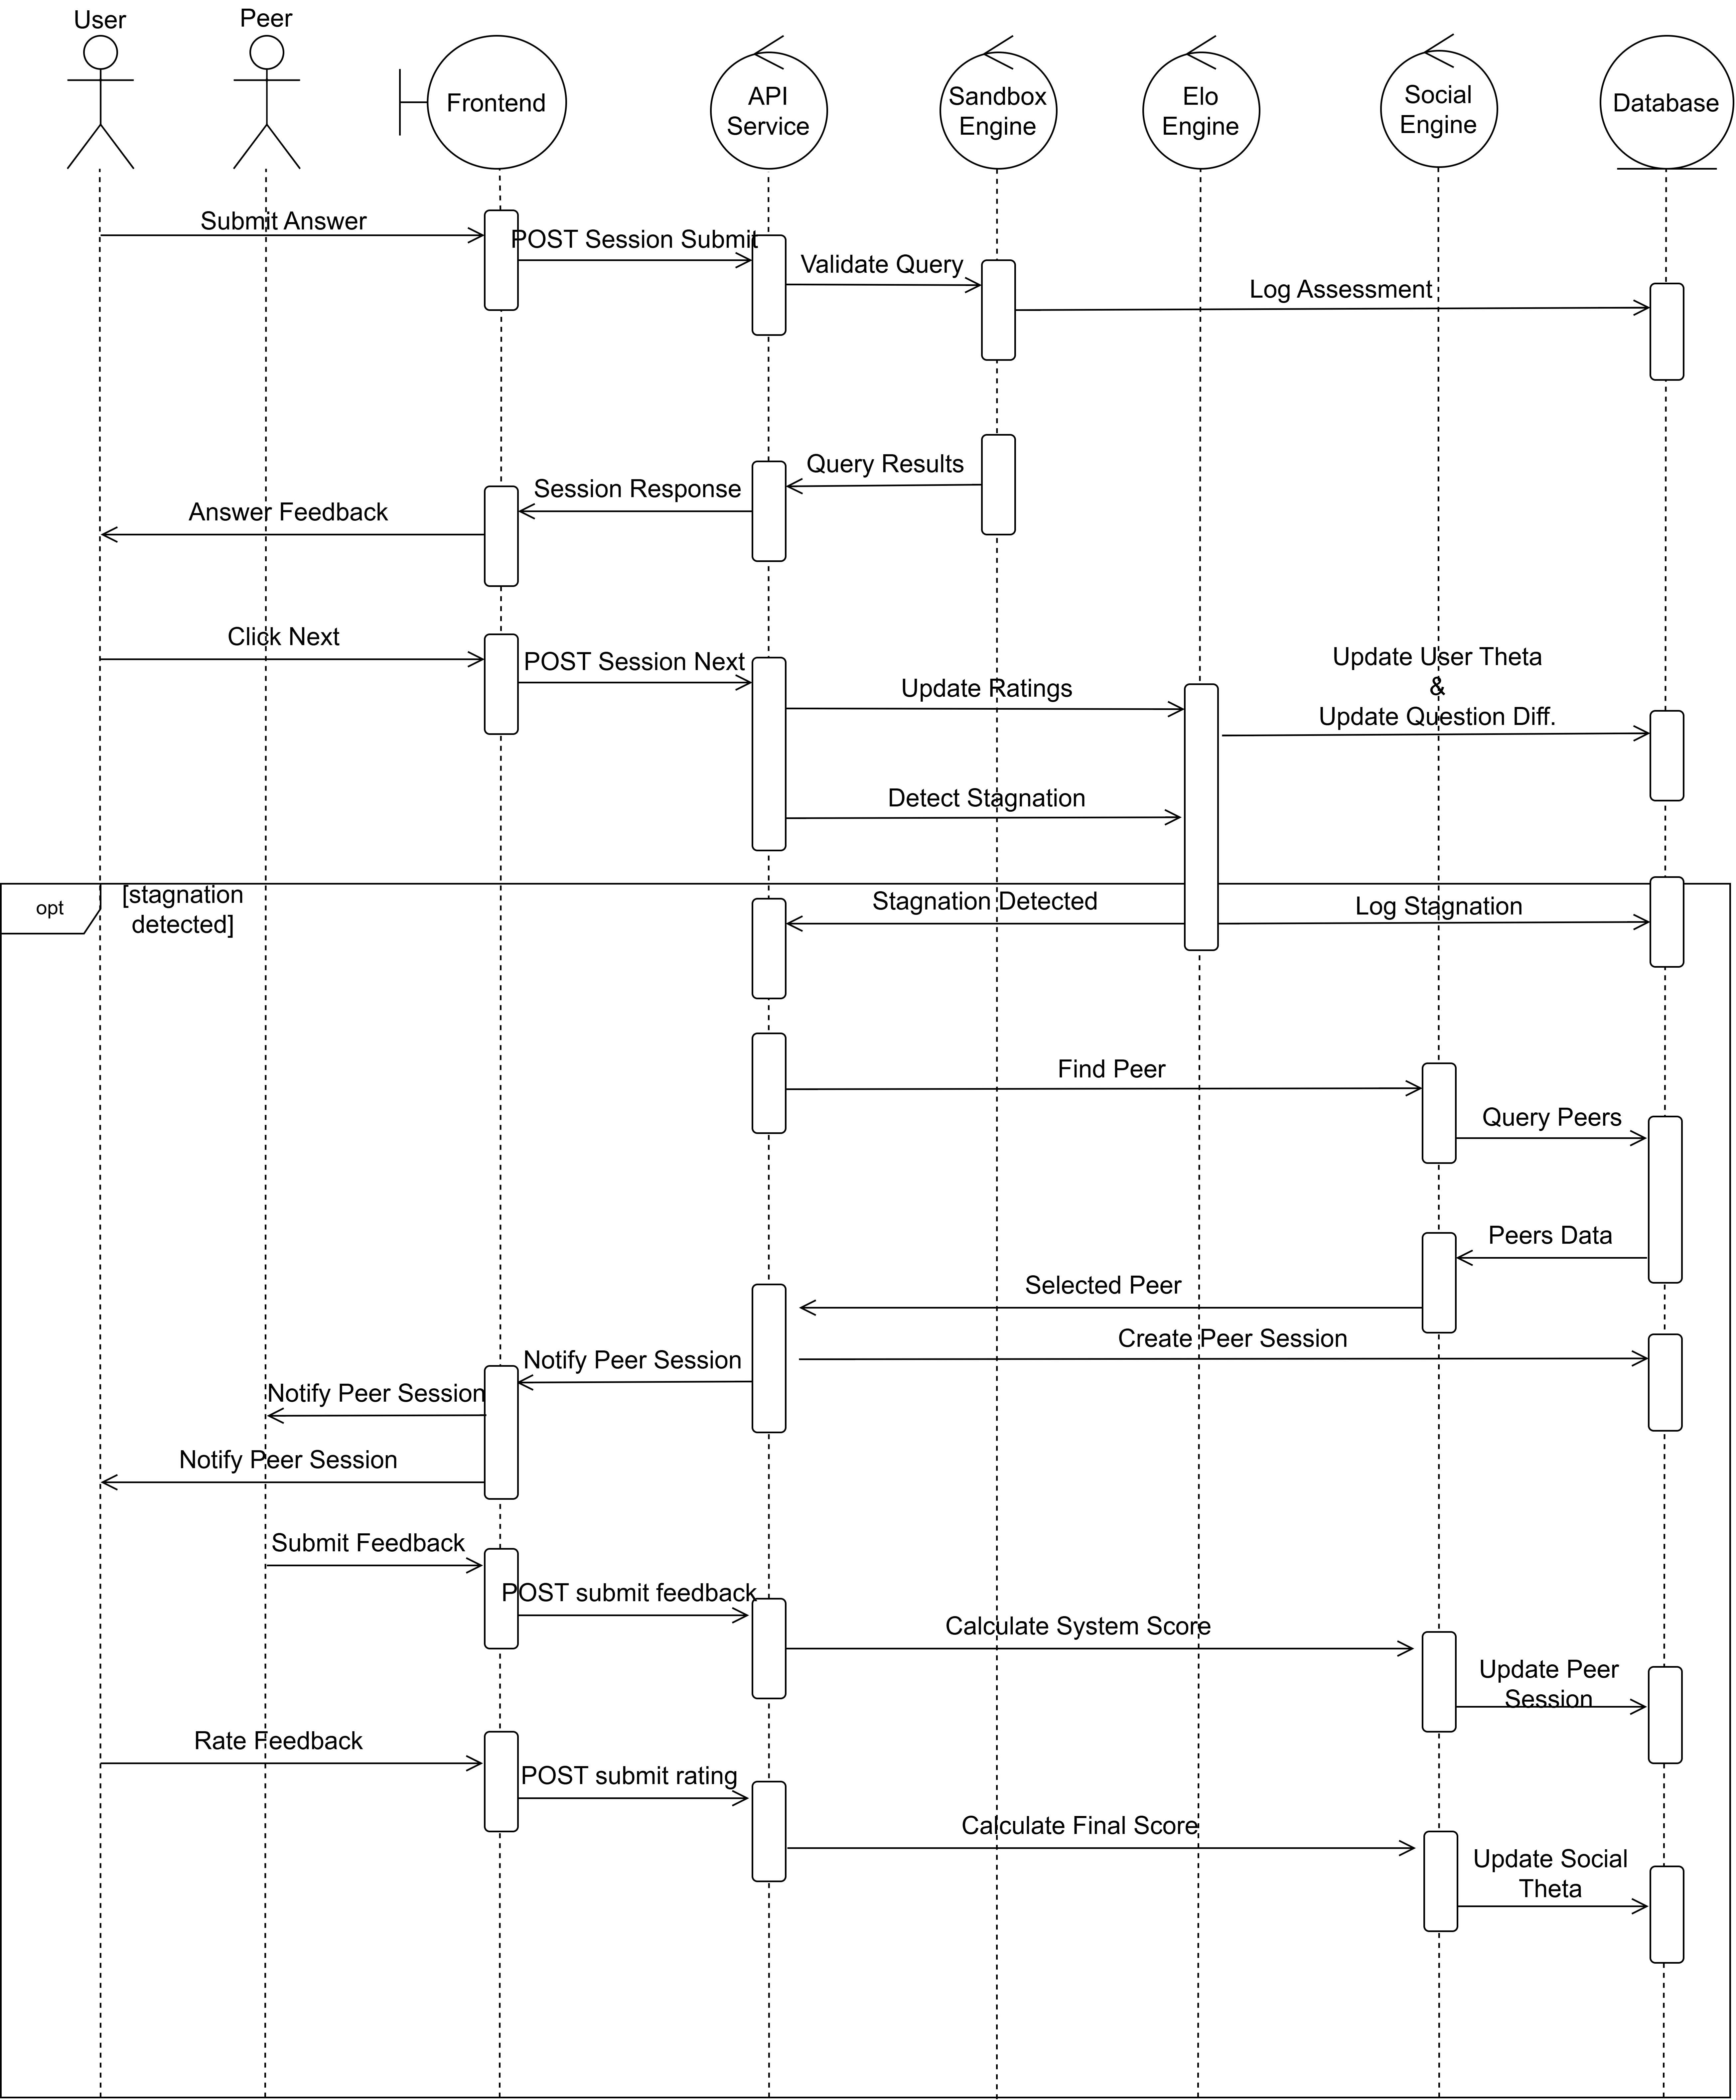
\includegraphics[width=0.9\textwidth]{images/sequence_diagram.png}
    \caption{\textit{Sequence Diagram} - Alur Interaksi Detail Sistem Asesmen}
    \label{fig:sequence_diagram}
\end{figure}

Alur interaksi teknis pada diagram di atas dapat diuraikan sebagai berikut:
\begin{enumerate}
    \item \textbf{Evaluasi Pengerjaan Soal:}
    Pemelajar (\textit{User}) mengirimkan jawaban melalui \texttt{Frontend}, yang kemudian diteruskan sebagai \texttt{POST Session Submit} ke \texttt{API Service}. Lapis layanan ini memanggil \texttt{Sandbox Engine} untuk memvalidasi kueri SQL yang dikirimkan. Setelah dievaluasi, log hasil pengerjaan dicatat ke dalam \texttt{Database}, dan hasil akhir dikembalikan secara berjenjang hingga \textit{User} menerima umpan balik jawaban (\textit{Answer Feedback}).
    
    \item \textbf{Pembaruan Kemahiran dan Deteksi Stagnasi:}
    Ketika pemelajar melanjutkan ke tahap berikutnya (\texttt{Click Next}), \texttt{API Service} memicu pembaruan (\texttt{Update Ratings}) ke \texttt{Elo Engine}. Algoritma ini akan memperbarui tingkat kemahiran pemelajar (\textit{User Theta}) dan tingkat kesulitan soal (\textit{Question Diff.}) di dalam \texttt{Database}. Setelah skor diperbarui, \texttt{API Service} memicu evaluasi stagnasi (\texttt{Detect Stagnation}). Jika \texttt{Elo Engine} mendeteksi stagnasi, status \textit{Stagnation Detected} dikembalikan, lalu kejadian ini dicatat (\texttt{Log Stagnation}) ke dalam \texttt{Database}.
    
    \item \textbf{Blok Opsional: Intervensi Sosial (\textit{opt [stagnation detected]}):}
    Jika kondisi stagnasi terpenuhi, alur eksekusi akan masuk ke dalam blok opsional yang memicu intervensi kolaboratif:
    \begin{enumerate}
        \item \textbf{Pencarian Rekan (\textit{Peer Matching}):} \texttt{API Service} memerintahkan \texttt{Social Engine} untuk mencari rekan (\texttt{Find Peer}). \texttt{Social Engine} menarik data kandidat dari \texttt{Database} (\texttt{Query Peers}) untuk mencari pasangan yang heterogen. Setelah rekan terpilih (\texttt{Selected Peer}) dikembalikan, sesi penilaian sejawat dibuat di \texttt{Database} (\texttt{Create Peer Session}). Notifikasi keterlibatan sesi kemudian disebarkan kepada \textit{User} yang bersangkutan dan \textit{Peer} yang terpilih.
        \item \textbf{Penilaian Sejawat (\textit{Peer Assessment}):} Aktor \textit{Peer} memberikan ulasan/umpan balik melalui \texttt{Frontend} (\texttt{Submit Feedback}). Data ini diteruskan ke \texttt{API Service}, yang kemudian memanggil \texttt{Social Engine} untuk mengevaluasi kualitas reviu secara otomatis (\texttt{Calculate System Score}) dan menyimpannya di \texttt{Database} (\texttt{Update Peer Session}).
        \item \textbf{Resolusi dan Evaluasi Umpan Balik:} Aktor \textit{User} membaca ulasan dari rekannya dan memberikan penilaian manfaat (\texttt{Rate Feedback}). Penilaian ini diproses oleh \texttt{API Service} dengan meminta \texttt{Social Engine} untuk mengalkulasi skor akhir (\texttt{Calculate Final Score}). Siklus ini ditutup dengan pembaruan tingkat kemahiran sosial (\texttt{Update Social Theta}) ke dalam \texttt{Database}.
    \end{enumerate}
\end{enumerate}

\section{Perbandingan dengan Sistem Saat Ini}
\label{sec:perbandingan}

Berdasarkan pemodelan konteks, interaksi, struktur, dan perilaku yang telah diuraikan, Tabel \ref{tbl:perbandingan_sistem} merangkum transformasi fundamental dari desain sistem konvensional yang dibahas pada Bab \ref{chap:studi-literatur} (\textit{As-Is}) menuju sistem yang diusulkan (\textit{To-Be}).

\begin{table}[!ht]
    \centering
    \caption{Perbandingan Desain Sistem \textit{As-Is} vs \textit{To-Be}}
    \label{tbl:perbandingan_sistem}
    \begin{tabular}{|p{0.20\textwidth}|p{0.37\textwidth}|p{0.37\textwidth}|}
        \hline
        \textbf{Dimensi Komparasi} & \textbf{Sistem Saat Ini (As-Is)} & \textbf{Sistem Usulan (To-Be)} \\
        \hline
        \textbf{Paradigma Interaksi} & 
        \textbf{\textit{Sistem pasif:}} \newline
        Sistem menunggu inisiatif siswa untuk berkolaborasi. Fitur sosial (forum/diskusi) bersifat opsional dan terpisah dari alur belajar utama. & 
        \textbf{\textit{Sistem proaktif:}} \newline
        Sistem secara aktif menginterupsi alur belajar mandiri dengan tugas kolaboratif (\textit{mandated intervention}) ketika mendeteksi stagnasi, mengubah peran siswa menjadi responden aktif. \\
        \hline
        \textbf{Arsitektur Data \& Asesmen} & 
        \textbf{\textit{Pembaruan satu sumber:}} \newline
        Model pengetahuan siswa hanya diperbarui oleh satu sumber data: hasil pengerjaan tugas individu. Aktivitas sosial tidak dikuantifikasi menjadi metrik kompetensi. & 
        \textbf{\textit{Siklus pembaruan dua sumber:}} \newline
        Model profil siswa diperbarui dari dua jalur: (1) skor tugas individu (dominan), dan (2) kualitas reviu sejawat. Aktivitas sosial dikonversi menjadi dimensi kontribusi sosial yang menjadi komponen komplementer dalam pemodelan profil siswa yang komprehensif. \\
        \hline
        \textbf{Logika Rekomendasi} & 
        \textbf{\textit{Heterogenitas opsional:}} \newline
        Algoritma cenderung merekomendasikan konten yang "nyaman" (sesuai tingkat kemampuan), berisiko menciptakan \textit{competency bubble} dan kompetensi semu. & 
        \textbf{\textit{Heterogenitas secara Desain:}} \newline
        Algoritma \textit{Re-ranking} secara eksplisit memaksakan batasan statistik ($\alpha$) untuk menyuntikkan mitra belajar dengan perbedaan tingkat kemampuan yang signifikan berdasarkan indeks \textit{Effect Size} (seperti \textit{Cohen's d}), memecahkan isolasi melalui eksposur diversitas. \\
        \hline
        \textbf{Mekanisme Mitigasi Isolasi} & 
        \textbf{\textit{Kesadaran manual:}} \newline
        Mengandalkan kesadaran metakognitif siswa (misal: lewat grafik OSSM) untuk menyadari bahwa mereka perlu berinteraksi dengan orang lain. & 
        \textbf{\textit{Batasan terautomasi:}} \newline
        Menggunakan batasan algoritmik otomatis. Sistem tidak menunggu siswa "sadar", melainkan langsung mengubah antarmuka menjadi mode \textit{Peer Assessment} saat parameter stagnasi terpenuhi. \\
        \hline
    \end{tabular}
\end{table}